%\todo{Obcas se trochu hodi ten text rozdelit do vic souboru, je to pak prehlednejsi (a mensi overkill na editaci)}
\todo{predelat na spravny format pdf}
\todo{zeptat se na odkazy u obrazku a odkazy u FANN a URHO3D}

\chapter{Introduction}
\todo{prefrazovat, projit, vylepsit}
\label{chap:gf}

Magic has been a popular part of computer games since their beginning. In many games, magic has its own lore and laws that make it systematical. Great examples of a complexity of magical spells are games \emph{Magicka} and \emph{Magicka 2}, where player casts spells by combining eight elements \ref{fig:magicka}. For example, using only earth element results in a rock thrown at the enemy, but adding fire will create a classic fireball.
\begin{figure}[!htb]
  \centering
  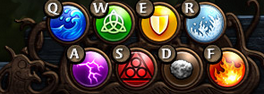
\includegraphics[width=0.5\textwidth]{ext/magicka.png}
  \caption{\emph{Magicka} spell interface}
  \label{fig:magicka}
\end{figure}

In books and movies, we can see wizards performing complicated hand gestures, or drawing on the floor some complex shapes. However, in games it is quite easy to do magic, since players often push a few buttons for even the strongest spells. This spoils the feeling of magic as something extraordinary and secret. We would like to allow developers to take a different approach, which requires players focus and concentration, as well as possible cooperation in spell casting.

While a majority of games binds spells to buttons, there are several games that used pattern recognition in their spell system. However, these systems recognized only simple gestures or patterns. Our goal is to make a more robust recognition system, that allows players to draw complex patterns.

\section{Pattern recognition in current games}

Since symbols and gestures are an integral part of the magic, there were many attempts to bring them into video game environment. \citet{gameMagic} provides a classification of gestural systems into three categories, which are overlapping, as sometimes combination of these approaches can be used. The following categories and facts are taken from \citet{gameMagic}.

\begin{description}
\item[Alternative controllers]
One such category are systems that utilize alternative controllers to mouse and keyboard, such as Kinect. Recent game from this category is \emph{Fable: The Journey}, where player casts spells by moving his hands. For example, push spell is cast by pushing into the air. Patterns made by the player are then recognized using Kinect technology. While moves are simple in nature, such as waving sideways or back and forth, both hands at the same time can be used, resulting in quite complex gestures.

\item[Restricted drawing forms]
Another technique used in several games is to let player draw into a predefined grid, or through predefined points. Both \emph{Castlevania: Dawn of Sorrow} and \emph{Deep Labyrinth} take advantage of an Nintendo DS drawing interface that allows players to draw magic signs. 
In \emph{Castlevania}, players draw signs by connecting glowing points in a circle in out-of-combat situations, as seen in \cref{fig:castlevania}. \emph{Deep Labyrinth} introduces special casting interface as well, consisting of 3x3 sized grid, where player connects dots. These approaches take away part of the freedom, but they make recognition algorithms much easier, e.g. by tracing only the order of points and selecting the right spell.

\begin{figure}
\centering
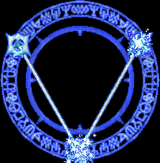
\includegraphics[width=.3\linewidth]{ext/castlevania.png}
\quad
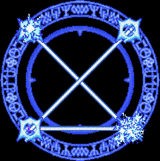
\includegraphics[width=.3\linewidth]{ext/castlevania2.png}
\label{fig:castlevania} %label se vaze na caption a musi bejt az po nem
\caption{\emph{Castlevania: Dawn of Sorrow} spell interface \XX{(image taken from ?)}}
\end{figure}

\item[Free-hand drawing]
To this category belong the examples that are most similar to our goal. One of the first games to integrate some form of pattern recognition of drawn shapes is \emph{Black \& White}, where the player takes a role of the god. Using a mouse, players are able to cast miracles by drawing a specific pattern onto the ground \ref{fig:blackwhite}. The player can draw anything anywhere on the ground, and its up to the game algorithm to recognize if it matches some of the miracle patterns. Alternatively, the player also cast miracle by clicking on a button, presumably because a lot of players had trouble drawing the miracles. 
A similar approach to recognition of player drawn spells and their recognition is used in \emph{Arx Fatalis}. Players are drawing symbols into the air with a mouse and the sequence of symbols represents some spell. While casting, game encoded the mouse moves into characters in 8-directions precision, each direction representing some letter. After player finished their spell, a Levenshtein distance was calculated from each predefined spell sequence to the user's created sequence and the candidate with the lowest Levenshtein cost was returned as a matching spell.

\begin{figure}
\centering
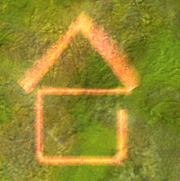
\includegraphics[width=.3\linewidth]{ext/gestureteleport.png}
\quad
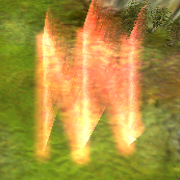
\includegraphics[width=.3\linewidth]{ext/gesturefireball.png}
\caption{\emph{Black \& White} teleport and fireball gestures}
\label{fig:blackwhite}
\end{figure}

\end{description}

\section{Goals}

We would like to allow players to draw complex spells. Instead of a sequence of symbols recorded over time, players could draw symbols arranged in a shape of another symbol, or embed one symbol in another. We also want our approach to be applicable in multi-player environments, where new situations can occur, such as multiple players drawing one spell. We don't want to introduce the aiding structures as in \cref{fig:castlevania} since they require and order in which they are passed and force the player to draw in a certain way or direction. They are also not very suitable for a multi-player environment since they can't handle multiple people drawing at the same time.

For the purpose of this work, we specify the following requirements that we have on our recognition system.
\begin{description}

\item [Durability against shape deformations]
Since we want to recognize hand-drawn shapes, our system has to be prepared for human-like imprecise drawing, especially when drawing with a mouse. However, defining what is deformed within some boundaries and should be recognized, and what is too deformed, is a difficult task.

\item [Extensibility]
We would like to offer an easy-to-use library that can be applied to other projects. For this purposes, we would like to let users define their own shapes that should be recognized. Our framework will offer interfaces for both preparing their own shapes and using them in the pattern recognition.

\item [Performance]
Our system should be applicable in demanding video games environment, prepared for the possibility of many players drawing their spells. To achieve this, we require fast recognition technique as well as usability in a parallel environment. 

\item [Recognition of embedded shapes]
To allow players cast complex spells, we need to give them an ability to somehow encode multiple symbols in one spell. One possible way to do it are shape embeddings. Each defined shape can contain several areas, where other shapes might occur. These areas are then processed in our recognition system and classified.

\item [Recognition of shape conglomerations]
For the purpose of this work, we consider shape conglomeration a group of shapes from the same shape class e.g. circle, arranged such that the whole conglomeration forms another shape. We can also look at it as taking the curves of the shape, sampling them uniformly, and then replacing all the samples with the pattern shape.

\end{description}

\subsection{Approach} \todo{vypsat kde co najdu}
To achieve our goals, we divide the work into several steps. First, we choose a pattern recognition algorithm which best suits our needs from several reviewed algorithms. Then we modify it to recognize embedded shapes and shape conglomerations since this topic is not very well covered. We use our system in a simple game, but we try to utilize most of the abilities of our recognition system to demonstrate its functionality. Finally, we measure its performance. We focus on two aspects of our implementation: performance and recognition effectiveness.


\chapter{Pattern recognition}
In this chapter, we define the pattern recognition problem. We then describe several classes of algorithms that solve pattern recognition. In the next part, we review some of the algorithms, namely \emph{Normalized cross-correlation}, \emph{Shape matching and object recognition using shape contexts} and \emph{Matching of Shapes Using Dynamic Programming}. The last section is devoted to \emph{Artificial neural networks} as our chosen method for the implementation.

\section{Pattern recognition definition}
First, we need to define what is actually meant by pattern recognition. \begin{quotation}
The Pattern Recognition problem consists in determining a procedure that, on the basis of the attributes, excluding those that define the classification criterion assigns each entity to its proper class.
\end{quotation} \cite{formalMethods}
 Pattern recognition problem is a broad term for classification problems based on similarity of the features of classified objects, see \citet{formalMethods} for precise mathematical definition. We will focus more on the shape recognition problems category, which can be viewed as a subcategory of pattern recognition. A shape can be typically defined as an equivalence class under the group of transformations, and the problem is then to algorithmically approximate the human-like visual pattern recognition. 

\section{Algorithms classification}
There are variety of algorithms on pattern recognition and they can be categorized based on different features. Approach classes based on \citet{imageRecognition} are:
\begin{description}
\item [Statistical approach] Algorithms in this category rely on the underlaying probability model. The shape class is determined by its extracted features and the probability distributions of the shape belonging to each class. An example of such algorithm is a naive Bayess classifier.

\item [Nonmetric approach] This class contains decision tress, syntactic methods, and rule-based classifiers. The idea of these algorithms is that each shape can be decomposed into the simplest sub-patterns called primitives. These primitives are then viewed as a language and the shape class as a set of rules, from which the shape can be derived. However, the inference of the grammar rules from the training data is difficult and the detection of the primitives as well.

\item [Cognitive approach] Neural networks and support vector machines belong to this class. Neural networks are inspired by human brains. They can be described as massively parallel computation systems and they can learn complex input-output relationships. \begin{quotation} However, in spite of the seemingly different underlying principles, most of the neural network models are implicitly similar to statistical pattern recognition methods. \end{quotation} \cite{imageRecognition}

\end{description}

We can also divide the algorithms based on the creation process of the classifier into learning-based approaches and template-based approaches \cite{skeletonMatching}. In the learning-based approaches, pattern classifiers are obtained through training on classified samples. In the template based approaches, patterns are described by templates and the recognition problem transforms into searching for the best matching template for a given input image.

Another classification proposed by \citet{distanceTransform} divides the algorithms into three classes based on the level of preprocessing:
\begin{description}
\item Algorithms that use pixel values directly, e.g. correlation methods.
\item Algorithms that use low-level features such as edges and corners, e.g. distance transform method.
\item Algorithms that use high-level features such as identified objects or relation between the features, e.g. graph-theoretic-methods.
\end{description}

Given the amount of algorithms to choose from, we have decided to describe only a few of them, namely normalized cross-correlation, shape contexts object matching and matching of shapes using dynamic programming, which are described on this chapter. Then we dedicate the whole chapter to neural networks, which we use in our algorithm implementation.

\section{Normalized cross-correlation}
Following description is taken from the work of \cite{crossCorrLewis}.
Cross-correlation is a method to measure the similarity between a template and a given area of an image. The term cross-correlation itself means a difference between two signals. Its one of the oldest approaches to pattern and feature recognition and extraction, and still serves as a base for more complex algorithms.
We compute an Euclidean distance of a image f and a template t, where pattern is on a position $(u\,v)$, by comparing corresponding pixels of the image at $(x\,y)$ and the template shifted to $(x-u\,y-v)$. 
\begin{equation*}
d_{f,t}^{2}(u,v)=\sum_{x,y} [ f(x,y) - t(x-u, y-v) ]^{2} 
\end{equation*}
When expanded, it gives us three terms. One of them is the cross correlation term $c(u,v)$.
\begin{equation*}
d_{f,t}^{2}(u,v)=\sum_{x,y} f(x,y)^{2} - 2c(u,v) + \sum_{x,y} t(x-u, y-v)^2
\end{equation*}
\begin{equation*}
c(u,v)=\sum_{x,y} f(x,y) * t(x-u, y-v).
\end{equation*}

Other two terms express energy (brightness) of template and image, respectively. We perform this computation for all possible values of u,v looking for the lowest value. Computing distance this way has several serious drawbacks. It is computationally heavy, it may give false matches if the image energy changes a lot with the position. Also, the range of values of cross-correlation term depends on the size of the template and it is not invariant to scaling and rotation. 

The slow performance of the method can be partially solved by computing the cross-correlation in a frequency domain using some form of a signal transform. Fourier transform is the common one, but other transformations were discovered, such as the wavelet transforms \cite{patternRecNN}. 
Convolution theorem states that when all conditions are met, Fourier transform of a convolution is an element-wise product of Fourier transforms of input signals. From Convolution theorem follows that time domain or space domain convolution is equivalent to element-wise multiplication in the frequency domain. To compute convolution, we simply need to take element-wise multiplications of Fourier transforms of signals to be convoluted. Cross-correlation differs in that we take the complex conjugate of the Fourier transform of the second signal.
Problems with the range of cross-correlation value and dependency on brightness can be fixed by using normalized cross-correlation, where image and template vectors are normalized to unit length. Other desired aspects, such as scale invariance, has been addressed in many algorithms using a cross-correlation method. However, they usually introduce some trade-offs and they may not achieve all the required properties together. 

Normalized cross-correlation:
\begin{equation*}
\gamma(u\,v) = \frac{\sum_{x\,y}f(x\,y) [f(x\,y)-\bar{f}_{u\,v}][t(x-u\,y-v)-\bar{t}]} {\{ \sum_{x\,y}f(x\,y) [f(x\,y)-\bar{f}_{u\,v}]^2 \sum_{x\,y}[t(x-u\,y-v)-\bar{t}]^2  \}^{0.5}}
\end{equation*}
where $\bar{t}$ is the mean of the feature and $\bar{f}_{u\,v}$ is the mean of $f(x\,y)$ in the region under the feature \cite{crossCorrLewis}.

\section{Shape matching and object recognition using shape contexts}
Shape matching using shape contexts is usually based on extracted features, which generally introduces a more robust recognition of deformed images. In the reviewed algorithm from \Citet{simple}, we try to find corresponding feature points of an image and a template, and we attempt to compute their distance as a sum of errors of corresponding points.

We treat an image as a set of points, and we assume that each shape is represented by a finite subset of its points. We extract from both image and template a certain number of feature points, the paper advises about 100 points. They do not need to be key-points, such as maxima of curvature or corners. This allows us to use a simple extraction method like edge detection. In our algorithm, we might also represent players drawings directly as a set of edges. 

With feature points extracted, we need to find corresponding points. To do so, \citet{simple} introduces a shape context descriptor. For each sample point $p$, we can create a set of vectors originating from $p$ to all other feature points. Such a set of vectors represents positions of other sample points relative to the origin point. The more sample points we choose, the more is this shape descriptor exact.

However, such descriptor might be too detailed and too sensitive to intraclass variations. In the paper, they presented a more robust and compact shape descriptor. The idea is that for each point $p$, we compute coarse histogram by assigning other points to bins in polar coordinates with a center in $p$. [TODO polar coordinates image] Polar coordinates are more sensitive to points near p. We can then compute the cost of matching two pints as 

\begin{equation*}
C_{ij} =  C(p_{i}\,q_{j}) = \frac{1}{2} \sum_{k=1}^{K} \frac{(h_{i}(k) - h_{j}(k))^2}{h_{i}(k) + h_{j}(k)}
\end{equation*}

where $ h_{i}(k) $ and $ h_{j}(k) $ represent the K-bin normalized histogram at $p_{i}$ and $q_{j}$. Given a set of costs $C_{i,j}$ between all pairs of points $p_{i}$ and $q_{j}$, we need to find the best alignment, which means that we want to minimize the total cost of matching 
\begin{equation*}
H(pi) = \sum_{i} C(p_{i}\,q_{pi(i)}).
\end{equation*}
This can be solved in $O(N^3)$ time using the Hungarian method\cite{simple}. 

We can achieve scaling invariance by normalizing all radial distances by the mean distance, and rotation invariance is obtained when searching for the lowest cost among all permutations. according to the paper, this method is robust against small geometric disturbances.

\section{Matching of Shapes Using Dynamic Programming}
Another method proposed by \citet{convex} introduces an algorithm which uses dynamic programming combined with high-level features. Similarly to the previous algorithm, we try to compute a distance of template and image, but in a different way.

The algorithm requires that both shape and template are represented as a sequence of convex and concave segments, split by inflex points. The idea of the algorithm is to recursively merge segments using two grammar rules $CVC -> C$ and $VCV -> V$, where V denotes concave and C convex segment. Simultaneously, merging cost is computed using a merging cost function, and results are stored in the dynamic programming table, with additional information.

Rows and columns of dynamic programming table represent inflex points of shape and template, respectively. At the end of the computation, each field $F(i,j)$ contains the minimal cost of merging first i-1 segments of shape and j-1 segments of template. Minimum cost is computed as:

\begin{equation*}
g(i_{w},j_{w}) = min\{g(i_{w},j_{w}) + \phi(a(i_{w-1}|i_{w}), b(j_{w-1}|j_{w}))\}
\end{equation*}
where the minimum is over all possible values of 
\begin{equation*}
(i_{w-1}\,j_{w-1})  =  (i_{w} - 2m_{w} -1\, j_{w} - 2n_{w} - 1)
\end{equation*}
, where $m \geq 0$ and $n \leq 0$.
Since merging of convex and concave segments is not possible, merging always involves an odd number of segments. Dissimilarity cost function: 
\begin{equation*}
\phi(a(i_{w-1}|i_{w}), b(j_{w-1}|j_{w}))  =  \lambda MergingCost(a(i_{w-1}|i_{w}))  +
\end{equation*}
\begin{equation*} 
\lambda MergingCost(b(j_{w-1}|j_{w}))  +  DissimilarityCost(a(i_{w-1}|i_{w}), b(j_{w-1}|j_{w}))
\end{equation*}

where lambda value controls merging tendency. With lower value, merging is more encouraged. For shapes with much detail, it is practical to set higher values, otherwise, these details may be lost during merging. 
Since algorithm assumes, that first segments of shape and template are aligned and match, we may need to run the algorithm for all possible starting points of shape if we don't know the first segment beforehand.

Contrary to the previous algorithm, we now require the extraction of high-level features, we need to extract convex and concave segments in correct order. However, we obtain a matching algorithm that is independent of shape translation, scaling and rotation. We can also directly control invariance to deformations using the lambda parameter.

\section{Neural networks}
Neural networks are mathematical models inspired by a behavior of a biological nervous system \cite{bishop}. They have been successfully used to solve problems in many different areas, including image and pattern recognition. They can be used in problems, where we can't mathematically describe the solution given the instance of the problem, or doing so would be overly complicated. We have chosen a neural networks approach as a core of our system. They don't require feature extraction since they can learn it themselves. They also have a great ability to generalize, which has been used for the recognition of shape conglomerations.

\subsection{Neuron}
Artificial neural networks are structures built for parallel data processing. The basic network unit is a neuron \ref{fig:neuron}, which is characterized by its input and output connection weights, the activation function and a bias. The neural network is built from a number of connected neurons, usually in a layered structure, and the network learning can be characterized as a process of altering the weights of the connections between neurons and the biases of the neurons.

\begin{figure}
\centering
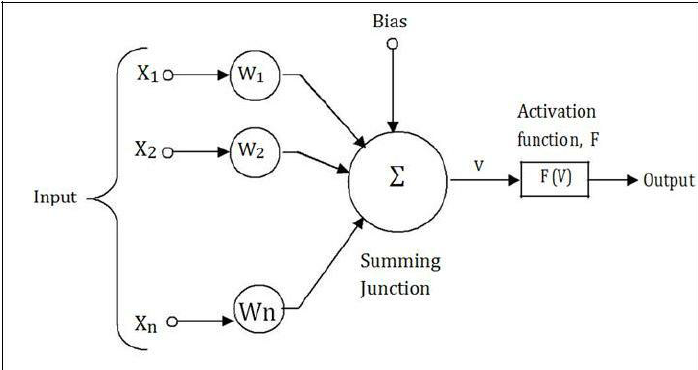
\includegraphics[width=.5\linewidth]{ext/neuron.png}
\label{fig:neuron}
\caption{The model of neuron unit}
\end{figure}

Activation function characterizes the behavior of the neuron. When the values from the input connections are computed, the activation function is applied onto the sum of the values and the result is passed further to other neurons. Common examples of activation functions are the step function and the sigmoid function.

\begin{description}
	\item [step function] $ x \geq 0: f(x) = 1; x < 0: f(x) = 0. $
	\item [sigmoid function] $ f(x) = \frac{1}{1+e^{-x}} $
\end{description}

\subsection{Artificial neural networks}
An artificial neural network is a mathematical model, consisting of a set of neurons interconnected by connections.
More exactly it is a set 
$M  =  (N,C,I,O,w,t),  where: $
\begin{description}
\item $N  is  a  finite  set  of  neurons.$
\item $C \subset N x N  is  nonempty  set  of  oriented  connections.$
\item $I \subset N  is  nonempty  set  of  input  neurons.$
\item $O \subset N  is  nonempty  set  of  output  neurons.$
\item $w : C -> R  is  weight  function.$
\item $t : N->R  bias  function.$
\end{description}

In practice, multilayer neural networks are commonly used. Multilayer networks are networks, in which neurons are organized in layers starting with the input layer and ending with the output layer, with hidden layers in between. For each neuron in this structure, its input connections originate only in a previous layer, and its output connections reach only to the following layer. 

\subsection{Learning process}
Learning process of an neural network is an optimization problem, where we want to optimize the error function. Error function describes a difference between actual and correct output values for given set of training data. One of the popular error functions is mean square error function:
\begin{equation*}
MSE = \frac{1}{n} \sum_{i=1}^{n} (Y_{i} - \hat{Y}_{i})^2.
\end{equation*}

Learning process consists of showing inputs to the network and adjusting its connection weights based on the actual and correct output values in order to lower the MSE.

\subsection{Learning algorithms}

\subsubsection{Back-propagation algorithm}
Back-propagation is one of the most popular algorithms for neural networks training, and it serves as a base for many other algorithms.

The algorithm is based on the gradient descent method. In the first step, the input is evaluated and the mean square error of the output is computed. However, a different error function may be used. We can compute the gradient $\frac{\partial E}{\partial w_{ij}}$ for a given training sample using the chain rule:
\begin{equation*}
\frac{\partial E}{\partial w_{ij}} = \frac{\partial E}{\partial in_{i}} \frac{\partial in_{i}}{\partial w_{ij}} = 
a_{j}*\frac{\partial E}{\partial in_{i}} = a_{j}*\frac{\partial E}{\partial a_{i}}*\frac{\partial a_{i}}{\partial in_{i}}
\end{equation*}
where $E$ is the error function, $w_{ij}$ is the weight of the connection between the neurons $i$ and $j$, $in_{i}$ is the weighted sum of the inputs of the neuron $i$ and $a_{i}$ is the output value of the neuron $i$.

If we use the sigmoid activation function denoted $g$, the derivation is:
\begin{equation*}
\frac{dg}{dx}  =  g(x)(1-g(x))
\end{equation*}
which gives us:
\begin{equation*}
\frac{\partial E}{\partial in_{i}} = a_{i}(1-a_{i}) \frac{\partial E}{\partial a_{i}}.
\end{equation*}
We can put the equations together to obtain:
\begin{equation*}
\frac{\partial E}{\partial w_{ij}} = a_{j} a_{i}(1-a_{i}) \frac{\partial E}{\partial a_{i}}
\end{equation*}
There we have two possible cases for the neuron $i$:
\begin{enumerate}
\item [1.] $i$ is an output neuron. Then we get: 
	\begin{equation*}
	\frac{\partial E}{\partial a_{i}} = -(t_{i} - a_{i})
	\end{equation*}
	where the $t_{i}$ is the expected output for the neuron $i$ for the current input.

\item [2.] $i$ is a hidden neuron. In this case we consider all neurons $k$ that recieve input from $i$. Since we are propagating backwards, we know the values $\frac{\partial E}{\partial a_{k}}$ for all $k$. Using chain rule again gives us:
	\begin{equation*}
	\frac{\partial E}{\partial a_{i}} = \sum_{k} \frac{\partial in_{k}}{\partial a_{i}} \frac{\partial E}{\partial in_{k}}
	\end{equation*}
and from combining the equations we get:
	\begin{equation*}
	\frac{\partial E}{\partial a_{i}} = \sum_{k} w_{ki}a_{k}(1-a_{k}) \frac{\partial E}{\partial a_{k}}
	\end{equation*}
\end{enumerate}
Now we have defined gradient values $\frac{\partial E}{\partial w_{ij}}$ for all weights in a given neural network.
We can then use the following rule to update the weights:
\begin{equation*}
\Delta^{t} w_{ij} = - \epsilon \frac {\partial E}{\partial w_{ij}} + \alpha \Delta w^{t-1}_{ij}.
\end{equation*}
$\Delta^{t} w_{ij}$ is the change at time $t$ for the weight $w_{ij}$. The value $\epsilon$ is called the learning rate. If the learning rate is too low, it will take much longer to train the network. If it is too high, the algorithm will cross large section in the search space and oscillate.

In summary, the input is evaluated and the difference between the correct and actual output is computed using error function. The difference is propagated back through the network and weights are updated using the gradient descent method. The whole process is repeated until the desired error value is achieved.

\subsubsection{Quick-prop algorithm}
The quick-prop algorithm is an improved version of the backpropagation. It is based on independent optimization steps for each weight, rather than updating all weights at once. For the update computation, it requires data from the last iteration, which increases space complexity. 

\begin{equation*}
\Delta ^{t} w_{ij} = \Delta^{t-1} w_{ij}*(\frac {\bigtriangledown_{ij} E^{t}} {\bigtriangledown_{ij} E^{t-1} - \bigtriangledown_{ij} E^{t}})
\end{equation*}
where $\Delta ^{t} w_{ij}$ is weight delta from \emph{t} iteration and $\bigtriangledown_{ij} E^{t}$ denotes partial $w_{ij}$-derivation of error function E in \emph{t} iteration.

\subsection{Convolution neural networks}
Convolution neural networks are a modern solution to image recognition. They are similar to classic neural networks, but the main difference is that they expect the input to be an image, and they allow us to encode some of the properties of images naturally into their architecture.

Neurons of convolutional networks have a layered architecture, like classic networks, but their layers consist of neurons arranged in a grid, similarly pixels of an image, and each neuron is connected only to a small corresponding area in next layer.  
TODO image

\subsection{Data preparation for pattern recognition}
\cite{bishop} Because of their generalization properties, neural network are successfully used in pattern recognition. They are able to approximate an arbitrary mapping between the input values and the output values. Because of this, we are not forced to do feature extraction and we can initialize the network with pixel values directly. 
It is however recommended to apply several pre-processing transformations that can improve the generalization performance significantly.
\begin{description}
\item [Input normalization]
One of the common forms of pre-processing is input normalization. By applying a linear transformation we can arrange all of the inputs to have zero mean and unit standard deviation over the transformed training set.
In practice, input normalization ensures that the inputs and target outputs stay in unit range, and we can expect that the weights should also be in unit range. We can then initialize the weights with suitable random number. Otherwise, we would have to find a solution, where the weight values differ distinctly.
\item [Training with noise]
Another technique that improves generalization is training with noise. It involves the addition of a random vector to the input vectors during training. in practice, it has been shown that training with noise can reduce over-fitting and improve network generalization.
\item [Data dimensionality reduction]
Data dimensionality reduction is a pre-processing method that actually results in fewer input neurons. It can be for example in the form of color information removal, or pixel averaging, where we group several pixel to one block and use average of each block as an input. By lowering the number of inputs, we lower the number of parameters that the learning process has to optimize.
\item [feature extraction]
Some of the more complicated techniques are based on feature extraction. Common are simple geometric primitives extractions, such as extraction of lines and their lengths, or angles. 
\end{description}

\chapter{Implementation}
In the first part of this chapter we describe the recognition system and in the second part we describe the game demo demonstrating the usage of the algorithm. Implementation of the recognition system consists of two parts, one responsible for the actual recognition, and one for the training of neural network based on user-defined shapes. The usage of the framework consists of three steps:
\begin{description}
\item[1.] defining the shapes and setting up desired recognition parameters.
\item[2.] training the neural network based using the defined shapes
\item[3.] using the framework and trained network to recognize patterns
\end{description}

\section{Data representations}
We have developed several data classes that are crucial for the algorithm to work. The first one is the class to represent input to the algorithm. The next class is a shape descriptor, an abstract class used to describe shapes, and the last one is a class for output data representation.

\begin{description}
\item [Image lines class]
First, we have to define the form of input. There are two general approaches to the representation of graphics data: vector graphics and raster graphics. Vector graphics data are usually more flexible, allowing us to perform deformations and scaling without loss of precision. They also take less space and can be converted into a pixel map when needed. On the other hand, they are harder to produce, since because they are built on the knowledge of mathematical relations in the image. 

Since we expect the input to the program to represent rather simple black and white shapes or their combinations, without any additional information like color or different shades, we have decided to create the interface for the vector graphics form of input.

The format of input is an instance of \texttt{ImageLines} class, defined in \texttt{ImageAnalyzer.h} header file. This class wraps a vector of lines defining the shape, accessible through \texttt{GetImageLines} method. The user is expected to fill the vector with the lines representing the two-dimensional image before passing it into the \texttt{Analyze} method. The class offers several other methods, used primarily by the recognition algorithm. 
A line is represented by the instance of class \texttt{Line}, whose constructor accepts two \texttt{float2} type vectors, first containing the start coordinates of the line, and second containing the end coordinates. Internally, the coordinates are transformed into three-dimensional vectors of a homogeneous coordinate system. 

\item [Shape descriptors]
Shape descriptors are a key part of the system, as they are used both during training of the neural network to produce shape examples and during analysis of image. They provide the algorithm with the information about the expected line positions and possible embedded shape locations. User can define their own shapes by inheriting from the abstract class \texttt{ShapeDescriptor} defined in \texttt{ImageAnalyzer.h} file. The shape descriptors use a parametric curves approach to define shapes. Abstract class functions, which should be defined by the user, take parameter \texttt{t} in the range $[0-1]$ as an argument, and return a point on the curve in a 2D space in the range $[0-1]^2$. The curve does not have to be continuous, but it has to return value for every parameter value in the range, and also thread safety of some methods is required. It is then recommended to keep the shape complexity low, as some very small details may be lost in the data preparation for the training. 

\item [Output data format]
Output is in the form of instance of \texttt{ShapeNode} class defined in \texttt{ImageAnalyzer.h} file. It represents a tree structure, where each node contains the recognized shape index, conglomeration shape index and embedded shapes as children. Indexes are numbers assigned to each descriptor during algorithm setup. \todo{podobny syntatickemu stromu}  \todo{schema}

\end{description}

\section{Recognition process}
The recognition process starts in the \texttt{Analyze} method, declared in the \texttt{ImageAnalyzer.h} file. It accepts an instance of \texttt{ImageLines} class as an argument, and returns \texttt{ShapeNode} instance describing the recognized elements in the image. The image lines are first normalized, which means transformed into the $[0-1]^2$ coordinate space. This transformation is essentially a rescaling, preserving the length ratio and angles. Then, the top level shape is analyzed by drawing the lines into the pixel map, which is then passed into the trained neural network as a vector of numbers. The highest network output is the matched shape pattern, but only if the value higher than a user-set constant. There are several more steps involved, described below:

\begin{description}
\item [Rotated shapes] If a recognition of a rotated shapes is enabled, the image lines are rotated user-defined times by an appropriate angle value, drawn and analyzed by the network at each angle. The network returns a vector of values, each value representing the similarity to the shape it represents, and the highest value is considered the matched shape. If there are several highest network outputs for different rotations with the same value, the first highest value among all outputs is considered. A recognized shape index is returned along with its matching rotation, in which it scored the highest network output.

\item[Compound shape]
When the top level shape is recognized, its shape descriptor is used to sample the theoretical curve points uniformly at the interval $[0-1]$. Then, for each sampled point, this point is expanded into a small square, the original image is clipped to this square, discarding the lines outside, and the result is analyzed recursively. Recognized shapes are counted over all samples, and if the count of matches for any shape is high enough, the top level shape is recognized as a compound shape created from a number of smaller shapes of the type with the highest count.Pattern shapes that form the composition are not tested for compound shapes.

\item [Embedded shape]
To recognize embedded shapes, we use the shape descriptor of the shape recognized previously, and focus on the embedded shapes locations. For each embedded shape location defined in the shape descriptor, we clip the image lines to that area, and recursively run the \texttt{Analyze} method on the result.

\end{description}

\section{Neural network preparation}
\todo{reference na FANN}
We use the \emph{FANN} neural network library to train and use neural networks. This open source software is easy to use and install while having a lot of options in terms of network architecture and training. Thanks to its simplicity, we were able to develop an automatized training system for the networks.

\subsection{Training data}
Training a neural network requires a training dataset. Since we want to allow the extensibility in the form of user defined shapes, we have two options. Either to let the user somehow make his own dataset, which is not very convenient, or generate the data procedurally and try to approximate human-like drawing. We generate the data based on the shape descriptors registered by the user. To generate a data sample for the neural network, we take the shape descriptor and create a \texttt{ImageLines} instance from it. It will be either a deformed simple shape instance or an instance of a compound shape. In the case of creating deformed simple shape instance, shape curve is sampled many times using the shape descriptor, and the points are connected by lines. 
To approximate the deformations each sample can be moved in the direction perpendicular to the line between the original position of the last point, and the original position of the the transformed point. \todo {picture}. The transformation  offset is linearly magnified and then reduced, resulting in a heuristics that try to approximate some of the humans like deformations of drawn shapes. Then, the line between the previous and new point is added to the image instance. In the case of the shape conglomeration, the shape curve is sampled much less frequently and each point is replaced by rescaled image lines of a randomly chosen shape, but this shape is the same for the whole composition.

\subsection{Training}
Training is done using the generated data from the previous methods and the \emph{FANN} library. First, the training data and test data are generated, where the size of training data can be changed by the user, and the size of the test data is one-third of the size of training data. Then the network is repeatedly trained on the training data until it reaches the user set up MSE, or until it stops improving. Internally, it starts with a high MSE target value, which is then gradually lowered, and in between the improvement ratio is checked. The algorithm used for training the network is called \emph{RPROP}, an improved version of the quickprop algorithm because we achieved best results with this algorithm in terms of the improvements stability. In the neural network, we use an \emph{Elliot} activation function.

\section{Game prototype}
The game, which demonstrates the usage of this pattern recognition work, has been developed using the URHO3D game engine in version 1.7\todo{cite}. \begin{quotation} Urho3D is a free lightweight, cross-platform 2D and 3D game engine implemented in C++ and released under the MIT license. Greatly inspired by OGRE and Horde3D. \end{quotation} It is easy to learn and use, and comes with many examples together with source codes of how to use it. It is built on a component-based scene model. 

\subsection{Game description}
The game is only a prototype to show the usability of the recognition algorithm. In the game, the player controls the character from a top down view perspective. The player can move and attack the enemies, but most importantly cast spells by drawing. Spells in the game are represented by totem objects, so each time the player casts spell, a totem is created. These totem have different effects on the characters, they can be positive effects that affect the player's character, like healing, or negative effects that affect enemies, like burning. The task for the player is to survive and destroy all the enemies in the game. Now we describe some of the constructs of the game implementation:

\begin{description}
\item [Drawable texture] \texttt{DrawableTexture} is a component attached to ground in the game. It allows player to draw shapes onto the ground. This component handles the lines sampling and glowing shape line nodes.

\item [Characters] The player's character and the enemies are represented by a composition of several components: the animated mutant model component, the health component and movement component. The enemies have also an AI component attached, while the player's character has an controller component attached which causes it to listen to the keyboard controls, and the caster component, which allows the character to extract the shape from the drawable texture, transforming the shape into an \texttt{ImageLines} instance for the recognition.

\item [SpellSystem] The \texttt{SpellSystem} component is a initialization component for the recognition algorithm. It is created only once for the game and the algorithm setup is situated in the constructor. It holds the shape indexes and is responsible for the algorithm output parsing and construction of the spell.

\item [Spell] An instance of a node with the spell component is created each time the player casts a spell. It is a temporary class, serving as a placeholder for the totem object. It invokes the algorithm's \texttt{Analyze} method in a separate thread and waits for the result. This way, the game doesn't freeze while the algorithm analyzes the image. The place of the totem is marked by a green fire while the image is analyzed. 

\item [Totem] The core of the game are totem objects and all the spell effects are represented by them. Each totem has a duration for which it exists and an area of effect around it, where the characters are influenced by its presence. The totem can have several effects to it attached.

\item [Effects]  Effects are components attached to the totems. When a character is inside an area of effect of the totem, the totem applies all of its effects on the character. However, the effects can also be of an single activation type, in which case they are activated only once when the totem is created. An example of such effect is increasing the totem duration.

\item [States] When an effect with duration is applied onto the character, a state component is attached to it. For example, when an over time healing effect is applied onto a character, the healing state component is attached to the character for a given duration.

\end{description}

\subsection{Spell system}
The game spell system consists of several parts. First is the \emph{DrawableTexture} component, which is attached to the ground entity. This component is able to track players drawings and store them as lists of points, each list representing one continuous line. When the player presses the button to cast the spell, the \emph{Caster} component attached to their character extracts the lines in a rectangular area around the character and transforms them into the vector of lines. Then the instance of \emph{Spell} class defined in the \emph{SpellSystem.h} file is created. There, the \emph{ImageAnalyzer::Analyze} method is finally called in a different thread and when the analysis is done, the result is parsed and the spell is cast.

\chapter{User guide}
\todo{Tohle je tradicne Appendix --- pro vlastni text prace to neni moc podstatny, krome toho ze tam chces nekam velice jednoduse (idealne v obrazku) popsat to API a rict proc je skvely, a pak se jen odkazes na appendix kde to vysvetlujes.}
\section{Recognition system}
\subsection{Creation of shape descriptor}
For the training as well as for the recognition, shape descriptors are required. The shape descriptors have several behavioral limitations, that need to be followed by the user. The intended purpose of the descriptor is to describe a single 2D shape in a $[0\,1]^2$ rectangular area. The descriptor is expected to return the same shape every time, without any modifications, and all of its methods should return the same values when called with the same parameters. It is also required, that all of the shape descriptor methods are thread safe. It is then recommended to design the shape descriptor as a class with a constant inner state. Not following these rules may result in the unexpected and dysfunctional behavior of the system. The user can create a shape descriptor by including the \texttt{ImageAnalyzer.h} header file and inheriting from the class \texttt{ShapeDescriptor}. This class contains several abstract methods, that should be implemented:
\begin{description}
\item[\texttt{GetName()}] Returns the name of the shape a string. This is only for debugging purposes and it does not have to be unique or even constant. However, it is recommended to return a constant unique name among the descriptors.

\item[\texttt{GetPoint(\texttt{float} t)}] Function overload with one parameter \texttt{t} returns a point of the curve, based on the \texttt{t} parameter. It is recommended to normalize the parameter into $[0\,1]$ range by \texttt{NormalizeParam} function.

\item[\texttt{GetPoint(float last\_t, float t, float point)}] Function overload with three parameters, that allows the descriptor to describe noncontinuous curves. The \emph{point} parameter passed by reference should be filled with the same value as from \texttt{GetPoint(t)} as it describes the point of the curve. Then the function should return true if the curve is continuous on the interval $[last_t\, t]$, otherwise false.

\item[\texttt{GetPointsOfInterest()}] Function, that describes places, where an embedded shape may appear. It returns a vector of \texttt{float3} type, where the first two numbers denote the top left corner of the square area, and the third number is the size of the square.
\end{description}

Examples of shapes descriptors can be found in the \texttt{ExampleShapeDescriptors.h} file.

\subsection{Algorithm properties}
There are several variables then can be set up and influence the functionality of the software. They can be found in the \emph{ImageAnalyzer} namespace. Some of them are used both in the training and in the recognition. It is necessary then for the user to be consistent and use the same settings for the recognition as they used for the training.

\todo{tosamy, enumerate vs. description, taky sem to predelal aby me nebolely voci :D }
\begin{description}
\item[\texttt{DEBUG\_IMAGE\_SAVE}] Boolean variable with default value false. If true, the images created during the recognition are saved as BMP files onto the hard disk, but only in the initial rotation of the image.

\item[\texttt{COMPOSED\_SHAPES\_ENABLED}] Boolean variable with default value true. If false, recognition algorithm recognizes the whole shape but does not search for the pattern shape that might compose it. During training, the examples generating algorithm does not produce compositions of the shape, so the network is not trained to recognize the composed shape.

\item[\texttt{COMPOSITION\_SAMPLES\_COUNT}] Integer variable describing the amount of samples taken when searching for the pattern shapes. This variable has no effect when composed shapes are disabled.

\item[\texttt{COMPOSITION\_WINDOW\_SIZE}] Float variable that describes the size of the sampling window used during composition matching. The actual window is a square with a side size of 2*\texttt{COMPOSITION\_WINDOW\_SIZE}. This variable has no effect when composed shapes are disabled.

\item[\texttt{COMPOSITION\_SAMPLES\_LIMIT}] Integer variable describing the number of minimum pattern shape matches. If the count of the pattern shape matches is lower, the pattern shape is not recognized. This variable has no effect when composed shapes are disabled.

\item[\texttt{EMBEDDED\_SHAPES\_ENABLED}] Boolean variable with default value true. If false, recognition algorithm ignores the positions, where embedded shapes might be, and recognizes only the top level shape and its composing shape. During training, the generating algorithm will not generate embedded shapes, and the network will not be trained to filter out these locations, where they might appear.

\item[\texttt{ROTATIONS\_ENABLED}] Boolean variable with default value true. If false, recognition algorithm will not test different shape rotations for the best match, but will rather use the initial rotation. This variable does not have an impact on training since rotation recognition is not a task of the neural network.

\item[\texttt{ROTATION\_SAMPLES\_COUNT}] The amount of samples created when matching rotated shape. It directly determines the rotation step angle size, which is 360/\texttt{ROTATION\_SAMPLES\_COUNT}. This variable has no effect when rotations are disabled.

\item[\texttt{DEBUG\_OUPUT}] Integer variable with default value 1. Controls the amount of debug info of the recognition system. If set to 0 or lower, no debug output is produced. If set to value 1, prints recognized shape with its matching rotation and its composing shape, for the top level shape and each embedded shape. If set to 2 or higher, produces the same output as with value 1, but also all network outputs from the analysis are printed for all the rotations.

\item[\texttt{IMAGE\_SIDE\_SIZE}] Integer variable, controls the size of the images that are created during analysis. Every time there is an instance of \emph{ImageLines} class that should be analyzed by the network, the lines are drawn into the square pixel map of a size set by this variable. It is also directly connected with the network input layer size, which has to be the second power of this value. The default value is 32, which means that the neural network has an input layer of size 1024 neurons, and the images produced in the algorithm are pixel maps of $32*32$ pixels.

\end{description}

\subsection{Training phase}
Training the neural network consists of several steps. The first step is to set up the variables controlling the behavior of the recognition and training algorithms. By including the \emph{Training.h} file, the user can access the \emph{ImageAnalyzer} namespace for setting up the variables, and the \emph{Training} namespace for the training functions. After setting the variables, it is necessary to register the desired shape descriptors through function \emph{Training::RegisterShapeDescriptor}. This function takes a unique pointer to the shape descriptor as its parameter, and returns an instance of \emph{ShapeIndex} class. This class is only a wrapper over integers but it works as an identifier of the shape for the network. Then it is necessary to create an instance of \emph{TrainingCase} class, representing the trained neural network. The class takes a vector of integers as its parameter, where each number in the vector represents the number of neurons in one layer. 
//TODO simplify the interface, finish section

\subsection{Recognition phase}
When the neural network is ready, the user can set up the recognition system and use it in a game. Set up consists of several steps. It is necessary to load the neural network into the algorithm, using \emph{ImageAnalyzer::LoadNetwork} function, which takes string describing the path to the network as an argument. Then, the user has to register the same descriptors uses for the training of the loaded network again, together with the corresponding \emph{ShapeIndex} instance. Alternatively, the \emph{ShapeIndex} instance can be created given the order number of the corresponding shape descriptor when registered for the training. It is also necessary to set up the algorithm properties the same way they have been set up during network training. When these steps are done, the user can repeatedly call the \emph{ImageAnalyzer::Analyze} function to determine the shape hierarchy in the provided \emph{ImageLines} instance. The \emph{Analyze} function is thread safe, so many calls can be done at the same time. However, the set up has to be done synchronously and only once, before the first call of \emph{Analyze} function. 

\section{Game}
TODO

\chapter{Results}

\section{Neural networks performance}
For the correct functionality of the algorithm, it is required that the network is able to recognize the shapes. There are numerous parameters for the neural networks, like the training algorithm choice, architecture, activation function. Because it is not feasible to test every combination of the parameters, we have tested the influence of only a several of these parameters, with the following set up:
\begin{description}
\item [Network architecture] The networks had a layered structure, with two hidden layers.
\item [Training algorithm] resilient back-propagation, alias rprop.
\item [Activation function] The Elliot activation function, faster version of the sigmoid activation function, which is considered a standard used in most applications.
\item [Shape descriptors] We have used four basic shapes: square, circle, triangle, a water drop. 
\item [Data] The training data and the test data were generated by the developed generator. The training data consisted of 150 000 images with some shape, each shape had the same amount of examples and 50 000 images of random data without shape pattern. The test data consisted of 40 000 images of examples of shapes, and 20 000 images of random data.
\end{description}

The parameters that we have tested are these:
\begin{description}
\item [Number of neurons] We have tried several values of both layers. For the first hidden layer, we have tried 100, 200 and 300 neurons, and for the second hidden layer 10, 20 and 30 neurons. 
\item [The value of MSE] We have trained the networks at different levels of precision, with the target MSE values of 0.1, 0.07, 0.04 and 0.01.   
\item [Algorithm settings] The neural networks were trained for different combinations of algorithm settings, with embeddings and composition off and on.
\end{description}
The combinations of the parameters above gave us 3*3*4*4 = 150 trained neural networks to evaluate.

\section{Evaluation}
The networks were evaluated in the following scenario. For each of the combinations of embeddings and composition being turned on or off, the dataset of 1000 images were generated, with the same amount of examples for each shape. Then, the network was assigned a score computed as a sum of scores for each example. Score per example was one of following:

\begin{description}
\item [1] If the maximum of the outputs of the network is in the corresponding output neuron of the shape that is in the example.
\item [2] If the maximum of in the correct output neuron and is higher than 0.5.
\item [-1] If the maximum is in the wrong output neuron which corresponds to the different shape than the one in the image.
\end{description}

These rules mimic the usage of the network in the algorithm, where value above 0.5 is a match and only maximum is considered. From the rules follows, that each network could achieve from -1000 to 2000 score points. 

\section{Algorithm parameters optimization}
Plot in \cref{fig:simples_com} shows the measurements of algorithm performance for various parameters, as described in the legend. \todo{nasledujici patri do captionu toho figure! misto toho by chtelo rict co ten vysledek vlastne znamena --- napr. zjistili jsme ze je neco optimalni nebo ze neco se vylozene nehodi?}The X-axis represents score, the Y-axis represents final MSE of the network in training and each object represents a single network, with training parameters as described in the legend.

\todo{exportovat grafy jako pdf}
\todo{lepe popsat co v tom grafu je}
\begin{figure}
\centering
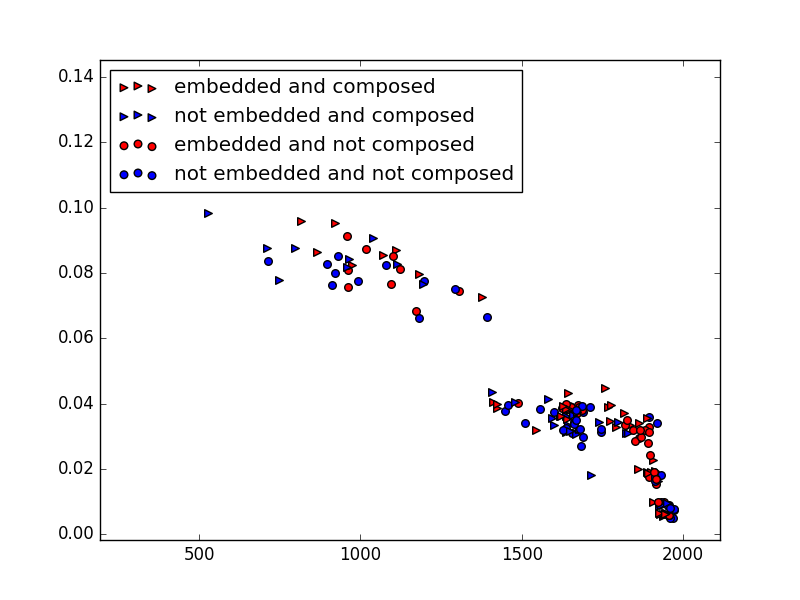
\includegraphics[width=.8\linewidth]{ext/figure_simples_com.png}
\caption{scores on data with simple shapes only, no embeddings and no composition}
\label{fig:simples_com}
\end{figure}

\begin{figure}
\centering
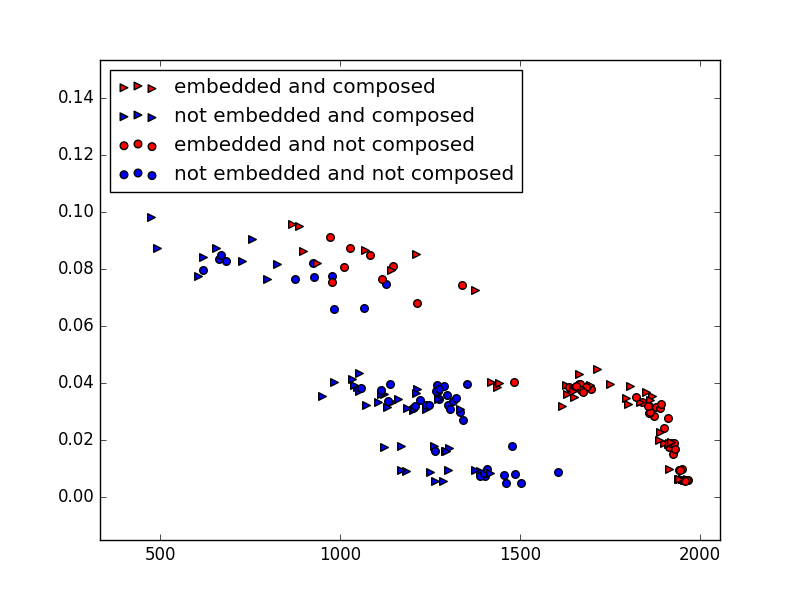
\includegraphics[width=.8\linewidth]{ext/figure_embed_com.png}
\caption{Scores on data with embeddings, no composition}
\label{fig:embed_com}
\end{figure}


\begin{figure}
\centering
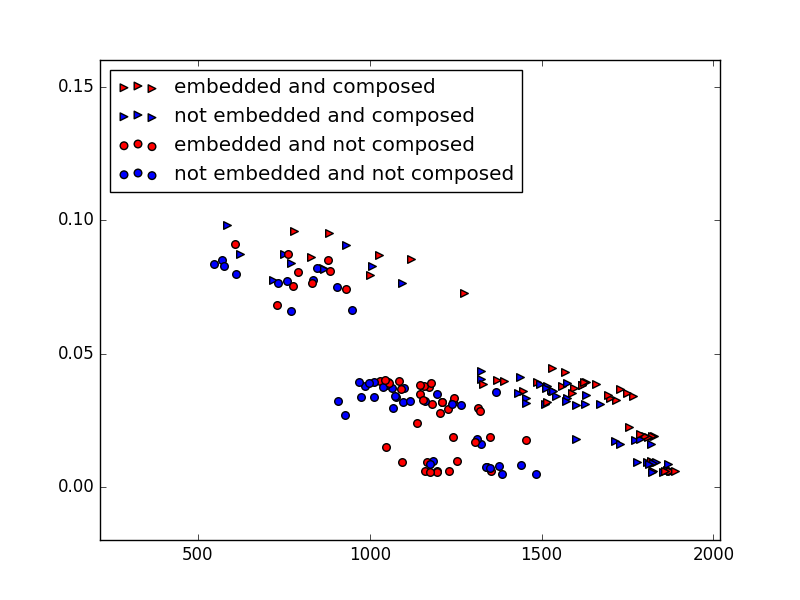
\includegraphics[width=.8\linewidth]{ext/figure_comp_com.png}
\caption{Scores on data with composition, no embeddings}
\label{fig:comp_com}
\end{figure}


\begin{figure}
\centering
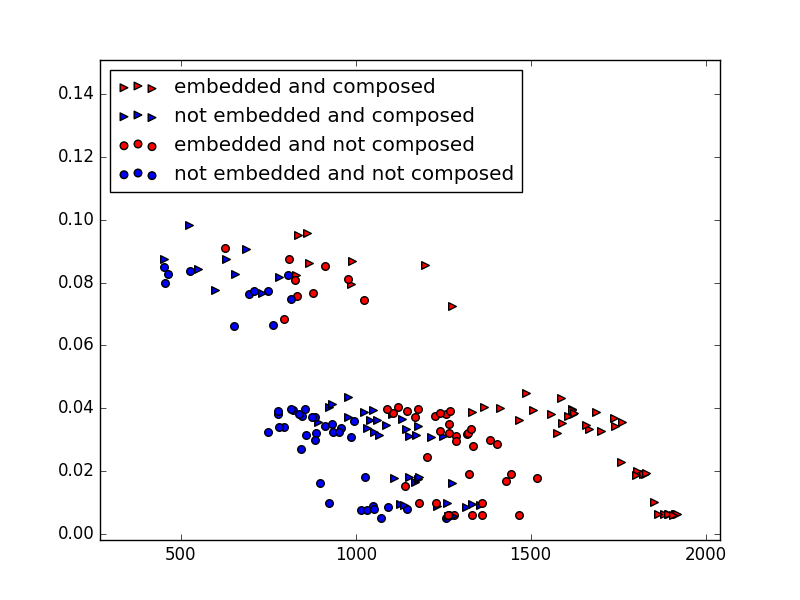
\includegraphics[width=.8\linewidth]{ext/figure_x_com.png}
\caption{Scores on data with both embeddings and composition combined}
\label{fig:x_com}
\end{figure}

From the \cref{fig:comp_com} \todo{it} is clear, that it is important to train the network for combinations of both embeddings and composition. More interesting is the observation from \cref{fig:simples_com} that turning on embeddings and composition affects the recognition of the simple shapes very slightly when reaching very low MSE. From the figures, it can also be observed, that the tendency to overtrain is not present and it is preferable to aim for lower MSE values in training.

\section{Network architecture}
\todo{opet: influence of the network architecture}
\Cref{fig:simples_arch,fig:embed_arch,fig:comp_arch,fig:x_arch} \todo{vsechny obrazky musi mit odkaz z textu, jinak ctenare nic nenuti na ne vubec kouknout :D} show the influence of different layer sizes on the overall performance of the network. Again, the X-axis represents score, the Y-axis represents final MSE of the network in the training and each object represents a single network, with the architecture described in the legend. Color represents the size of the first hidden layer, while shape represents the size of the second hidden layer.

\begin{figure}
\centering
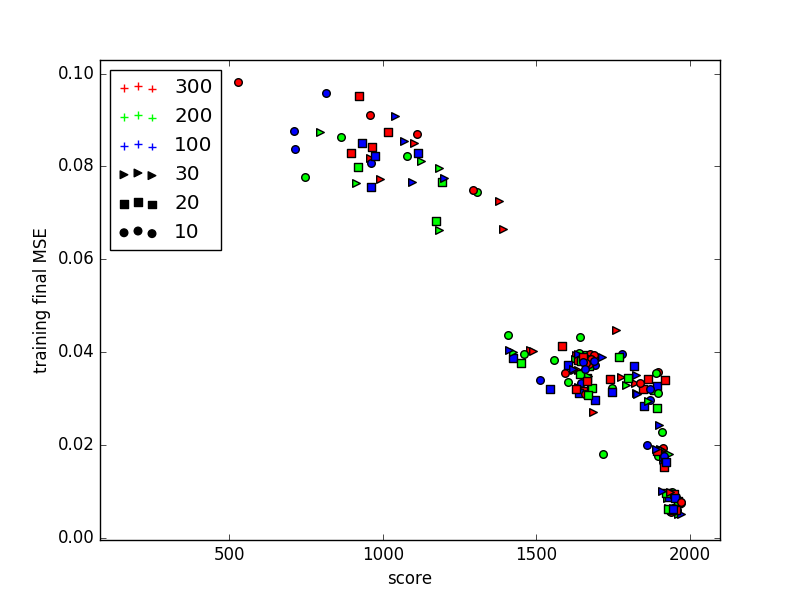
\includegraphics[width=.8\linewidth]{ext/figure_simples_arch.png}
\caption{scores on data with simple shapes only, no embeddings and no composition}
\label{fig:simples_arch}
\end{figure}

\begin{figure}
\centering
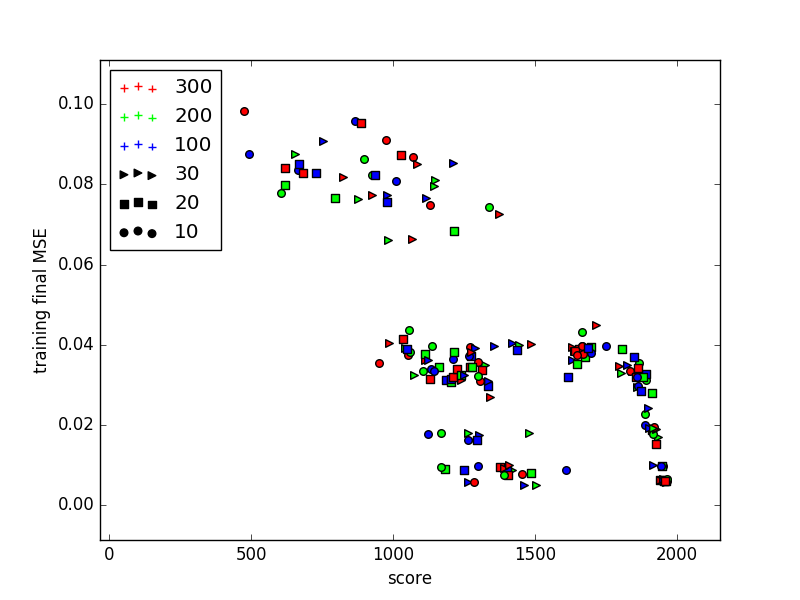
\includegraphics[width=.8\linewidth]{ext/figure_embed_arch.png}
\caption{Scores on data with embeddings, no composition}
\label{fig:embed_arch}
\end{figure}

\begin{figure}
\centering
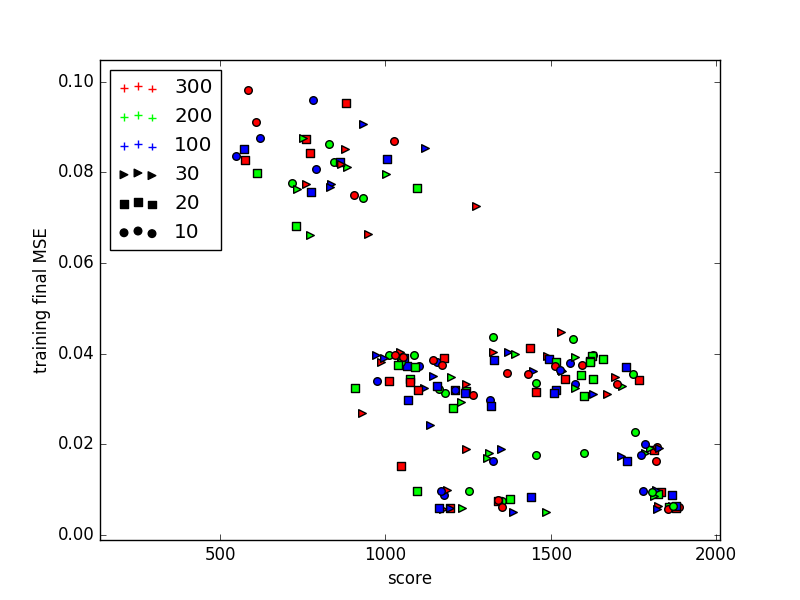
\includegraphics[width=.8\linewidth]{ext/figure_comp_arch.png}
\caption{Scores on data with composition, no embeddings}
\label{fig:comp_arch}
\end{figure}

\begin{figure}
\centering
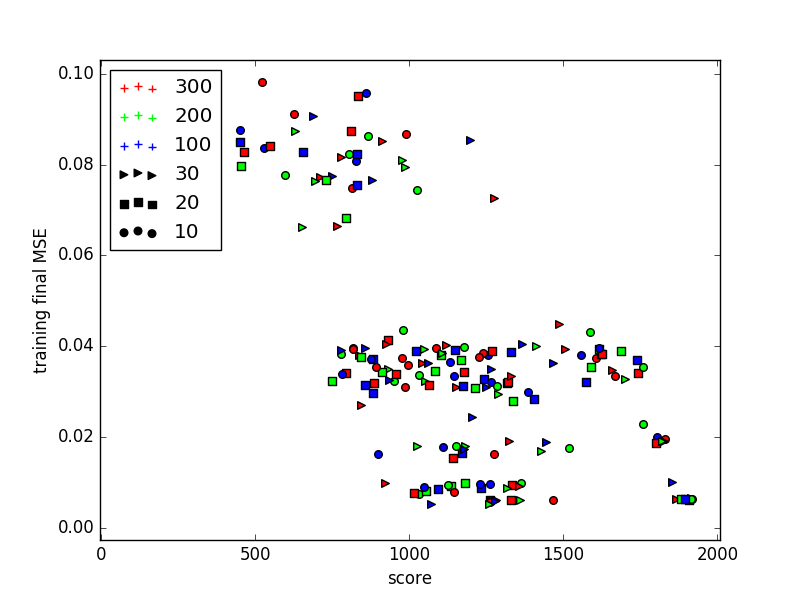
\includegraphics[width=.8\linewidth]{ext/figure_x_arch.png}
\caption{Scores on data with both embeddings and composition combined}
\label{fig:x_arch}
\end{figure}

The figures do not show any clear pattern. All the values used in the tests were able to achieve good results, even the network with the lowest number of neurons. It may be necessary to increase the number for a higher count of shape descriptors, but for the four used shape descriptors, even the 100-10 network was sufficient.

\section{Composition recognition}
To measure composition precision, we have prepared 100 \emph{ImageLines} instances of composition examples. Each instance represented a shape composed of examples of another shape. In the algorithm, we have used the best performing network trained for both composition and embeddings. Then we have analyzed the instances under the following set up:
\begin{enumerate}
\item \texttt{COMPOSED\_SHAPES\_ENABLED = true;}
\item \texttt{EMBEDDED\_SHAPES\_ENABLED = false;}
\item \texttt{ROTATION\_ENABLED = false;}
\end{enumerate}

\todo{tady odsud by to ty identifikatory chtelo vsechno dat do texttt}

We have tested different combinations of settings of variables COMPOSITION\_SAMPLES\_COUNT, COMPOSITION\_SAMPLES\_LIMIT and COMPOSITION\_WINDOW\_SIZE. We have compared the correct pattern shape with the recognized pattern shape for each test instance. The Y-axis shows the percentage of correct pattern shape recognitions and the X-axis shows a count of samples made around the shape contour. In \cref{fig:com,fig:com_speed} the COMPOSITION\_WINDOW\_SIZE is represented by the color and the COMPOSITION\_SAMPLES\_LIMIT by the shape. The COMPOSITION\_SAMPLES\_COUNT is on the X-axis. 
\begin{figure}
\centering
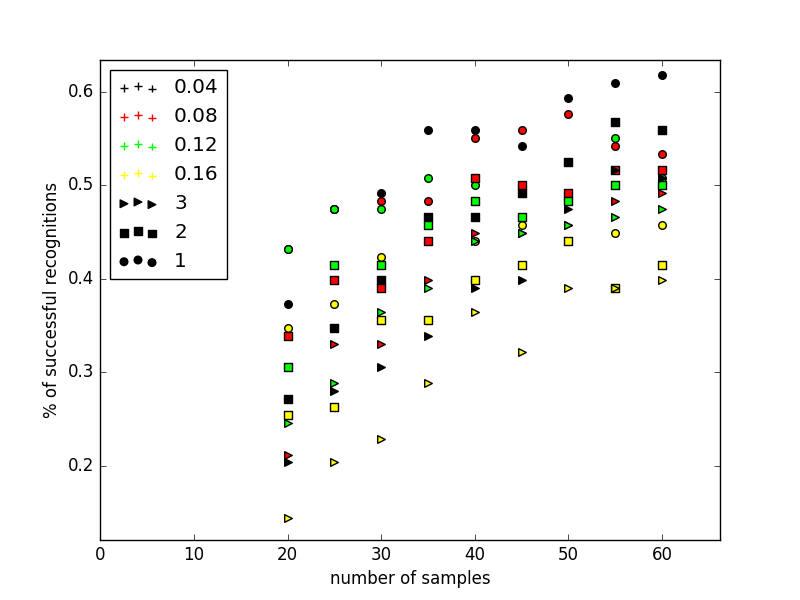
\includegraphics[width=.8\linewidth]{ext/figure_composition.png}
\caption{Precision of composition recognition. \XX{Jsou tady na ty ose Y fakt procenta? jestli jo tak 0.5\% neni vubec moc. :D}}
\label{fig:com}
\end{figure}

In \cref{fig:com}, we can see that success rate grows with the increasing number of samples. We can also see that the red and black colors representing the smaller sizes of the sample window perform better with the higher sample count. There is also a great drop in success rate when increasing the sample limit even by one. There are several factors that affect the recognition. The sampling window follows the ideal path from the shape descriptor, but the real shape is usually more or less deformed, which means that the window will hit only a part of the pattern shape. The pattern shapes can be of various sizes which is hard to approximate by the single size of the sampling window. And even the window hits the whole pattern shape, there is a very high chance of hitting also the noise from other shape patterns, or from embeddings. All these factors make the recognition for the network very difficult. From the shape locations in \cref{fig:com} we can deduce that the network is rarely able to recognize even a single pattern shape correctly, and after 40 samples, the success rate does not improve much and stays somewhere between 40\% and 60\%.

\begin{figure}[!htb]
\centering
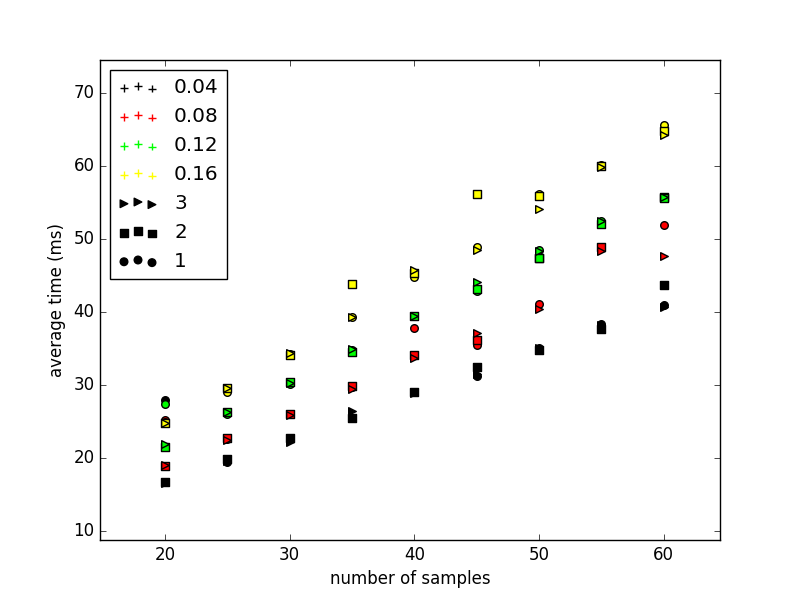
\includegraphics[width=.8\linewidth]{ext/figure_composition_speed.png}
\caption{Performance of composition recognition}
\label{fig:com_speed}
\end{figure}

It is clear that the algorithm becomes gradually slower with the increasing number of samples as shown in \cref{fig:com_speed}. The total time will also increase substantially if the rotation is turned on.

\section{Rotation}
Rotation invariance is achieved by redrawing the image at different angles and returning the best match from all samples [TODO ref description]. We tested the influence of the ROTATION\_SAMPLES\_COUNT on the precision and speed of the algorithm. In \cref{fig:rotation_simple_precision} we can see that the precision reaches a very high success rate at 15 samples and the computation time is linear to samples count and \todo{and what?} \cref{fig:rotation_simple_speed}. However, the performance of rotation recognition on composed shapes is much worse both in precision and computation time. From \cref{fig:rotation_comp_precision} we can see that the precision reaches about 70\% at 15 samples and improves only a little when we increase the samples count. The speed of recognition of composed shapes is slower by a magnitude in \cref{fig:rotation_comp_speed}. This is caused by the fact, that composed shapes contain a lot more lines than the simple shapes. We can deduce that setting ROTATION\_SAMPLES\_COUNT to higher than 15 is rather impractical.

\begin{figure}
\centering
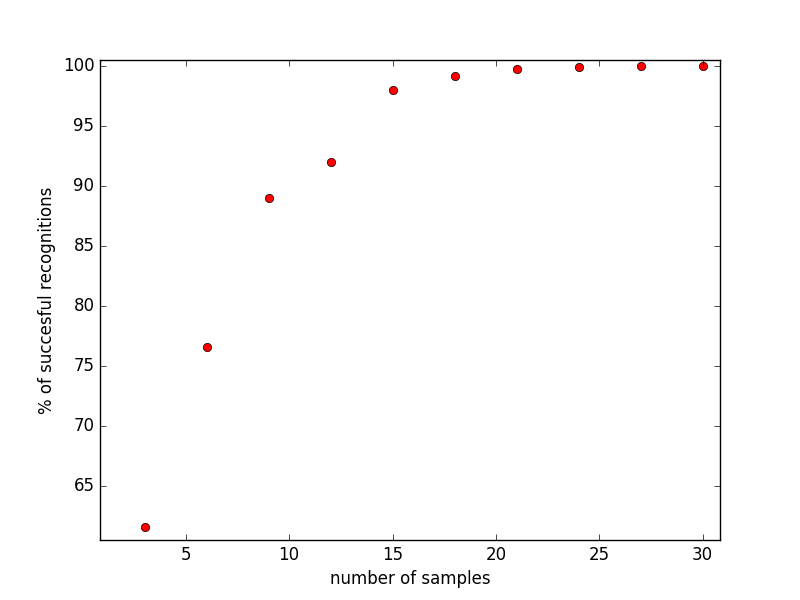
\includegraphics[width=.8\linewidth]{ext/rotation_simple_precision.png}
\caption{Precision of rotation recognition of simple shapes}
\label{fig:rotation_simple_precision}
\end{figure}

\begin{figure}
\centering
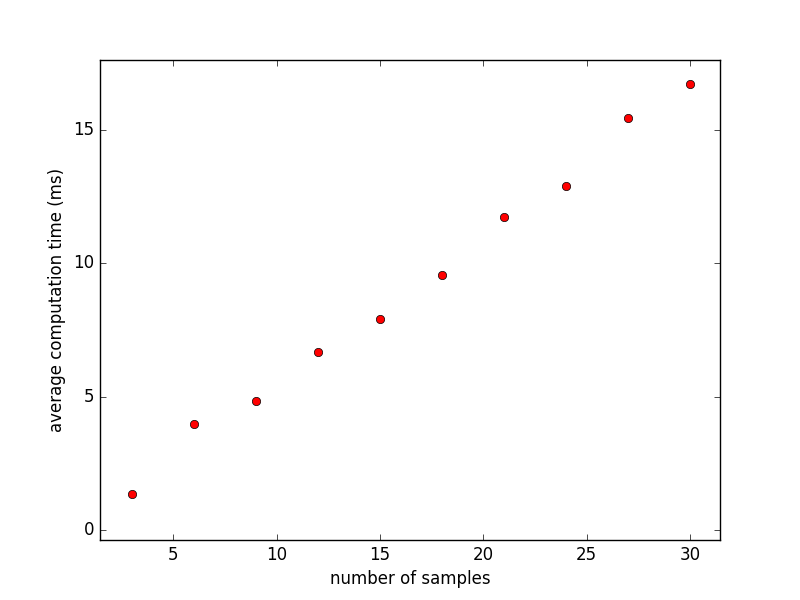
\includegraphics[width=.8\linewidth]{ext/rotation_simple_speed.png}
\caption{Performance of rotation recognition of simple shapes}
\label{fig:rotation_simple_speed}
\end{figure}

\begin{figure}
\centering
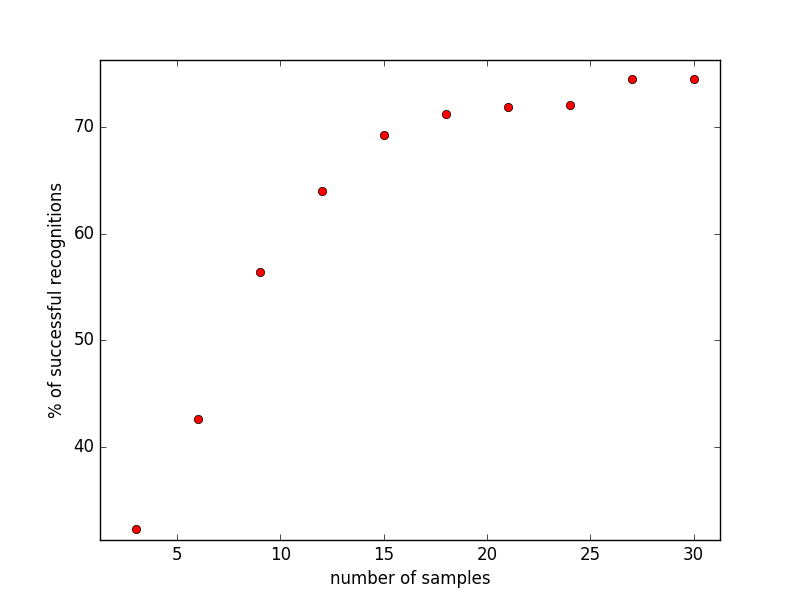
\includegraphics[width=.8\linewidth]{ext/rotation_comp_precision.png}
\caption{Precision of rotation recognition of composed shapes}
\label{fig:rotation_comp_precision}
\end{figure}

\begin{figure}
\centering
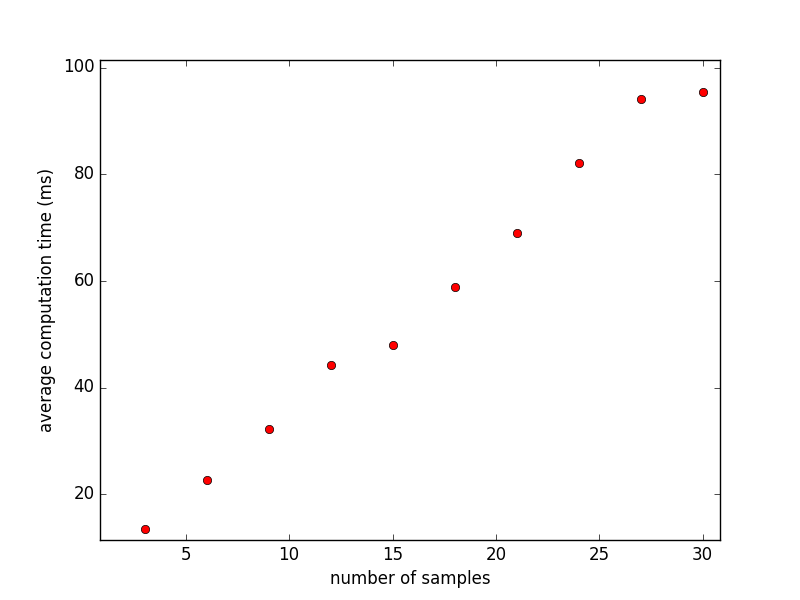
\includegraphics[width=.8\linewidth]{ext/rotation_comp_speed.png}
\caption{Performance of rotation recognition of composed shapes}
\label{fig:rotation_comp_speed}
\end{figure}

\section{Embeddings}
The ability of the algorithm to recognize embeddings depends on the shape descriptor definition. There the user can define the points of interest by their position and size. These two parameters form a rectangular area where the algorithm will search for embedded shape. It is then recommended to set the size of this area lower, to avoid fragments of the top shape appearing in this area, which might cause the network to not recognize the embedded shape. If the embeddings should appear in the composed shapes, the area should be even smaller, otherwise, the fragments of the pattern shapes will appear inside. The speed is influenced by the number of embeddings such that every point of interest if analyzed recursively.

\todo{Chces sem dat nekolik screenshotu ze hry ktery demonstrujou jak to nakonec vypada. Zaroven by nebylo spatny ukazat nejakej malej sample tech trenovacich a generovanejch dat, pripadne nejaky outliery (ty sou vzdycky zajimavy). Obecne by hodne prospel i zajimavej obrazek toho co presne vizualne znamena embedding a composition, hned k zacatku tyhle kapitoly.}
\todo{Diskusion jen pokud je potreba, jinak je to uz popsane vyse}

\chapter*{Conclusion}
\todo{2-3 odstavce, o tom co jsem udelal co neudelal vuci intru. v present perfect. future work, improvements. create game - turn based ideally alternativni pristup ke kompozicim - kreslit mysi neprakticiky, gpu pararelizace}

\todo{obrazky - ukazat co je conglomeration, pattern shape, embedded shape atd..}